\documentclass{article}
\usepackage{amsmath}
\usepackage{amssymb}
\usepackage[dvipsnames]{xcolor}
\usepackage{graphicx}
\usepackage{enumitem}
\usepackage{titling}
\usepackage{centernot}
\usepackage[margin=1.2in]{geometry}
\begin{document}

\setlength{\droptitle}{-7em}   % This is your set screw

\title{Algorithms Quiz \#4-5}
\author{Ozaner Hansha}
\date{April 28, 2020}
\maketitle

\subsection*{Problem 1}
For the following questions consider the following directed graph:
\begin{center}
  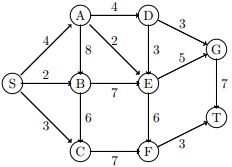
\includegraphics{graph.png}
\end{center}

\noindent\textbf{Part a:} Find the maximum flow from $S$ to $T$ by inspection.
\bigskip

\noindent\textbf{Solution:} The maximum flow from $S$ to $T$ is 9. Note that there is only $4+2+3=9$ capacity across all the outgoing edges of $S$, which means the flow cannot be any higher than 9. This combined with the flow of value 9 given in part b implies that 9 must be the maximum.
\bigskip

\noindent\textbf{Part b:} Show the amount of flow along each edge.
\bigskip

\noindent\textbf{Solution:} Below is a graph showing the flow along each edge for an optimal solution:
\begin{center}
  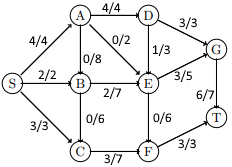
\includegraphics{graphFlow.png}
\end{center}
\bigskip
\newpage

\noindent\textbf{Part c:} Give the residual graph corresponding to the optimal flow.
\bigskip

\noindent\textbf{Solution:} Below is the corresponding residual graph of the optimal solution given in part b:
\begin{center}
  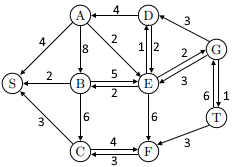
\includegraphics{graphResidual.png}
\end{center}
\bigskip

\noindent\textbf{Part d:} Give the minimum $(S,T)$ cut from the residual graph in part c.
\bigskip

\noindent\textbf{Solution:} The minimum cut is given by the following partition of $V$:
\begin{align*}
  L&=\{S\}\\
  R&=\{A,B,C,D,E,F,G,T\}
\end{align*}

Where $L$ is the set of vertices reachable from $S$ in the residual graph, and $R=L^\complement$. We can represent this graphically:
\begin{center}
  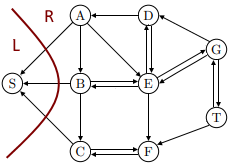
\includegraphics{graphCut.png}
\end{center}

\subsection*{Problem 2}
\noindent\textbf{Problem:} Convert the following CNF into a graph $G=(V,E)$ such that $G$ has a clique of size 4 iff the CNF is satisfiable:
$$\underbrace{(x_1\vee\overline{x_2}\vee x_3)}_{C_1}\wedge\underbrace{(\overline{x_1}\vee x_2\vee x_3)}_{C_2}\wedge\underbrace{(x_1\vee\overline{x_3})}_{C_3}\wedge\underbrace{(x_2\vee\overline{x_3}\vee x_4)}_{C_4}$$

Does $G$ have a clique of size 4?
\newpage

\noindent\textbf{Solution:} In the context of the clique problem, the given CNF corresponds to the following graph:
\begin{center}
  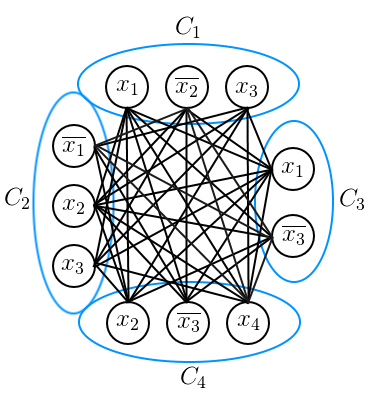
\includegraphics[scale=.8]{clique.png}
\end{center}

You'll note that many cliques of size 4 exist. We give one such clique below, highlighted in orange:
\begin{center}
  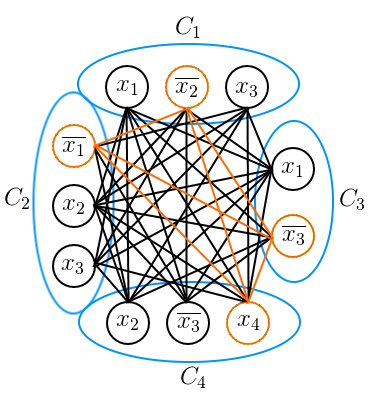
\includegraphics[scale=.8]{clique2.png}
\end{center}

\subsection*{Problem 3}
\noindent\textbf{Problem:} For the graph $G$ from problem 2, construct the complementary graph $\overline{G}=(V,\overline{E})$. What is the largest clique in $G$? What is the smallest vertex-cover in $\overline{G}$?
\bigskip

\noindent\textbf{Solution:} The complement $\overline{G}$ of the graph given in problem 2 is given below:
\begin{center}
  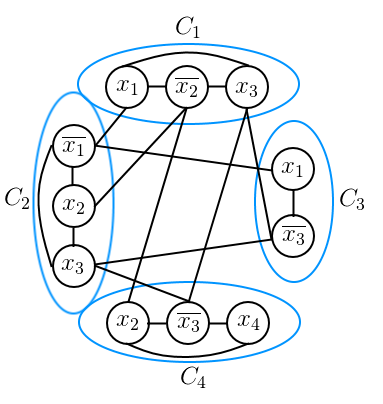
\includegraphics[scale=.8]{cover.png}
\end{center}

A maximal clique in $G$ of size 4 and a minimal vertex-cover in $\overline{G}$ of size 7 are both given below:
\begin{center}
  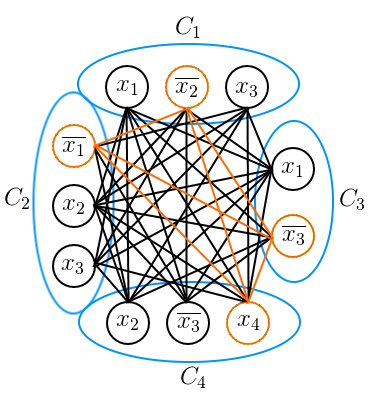
\includegraphics[scale=.6]{clique2.png}
  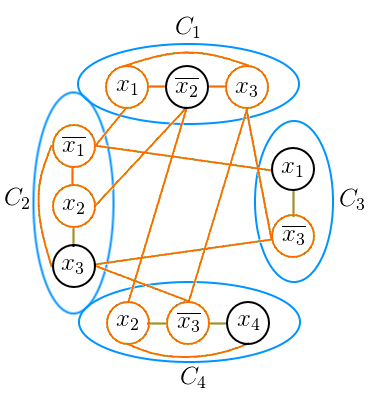
\includegraphics[scale=.6]{cover2.png}
\end{center}

To prove that 4 really is the maximal clique size of $G$, we simply have to note that no two vertices are connected within a clause. As such, no clique can have more than 1 member per clause, totalling a maximum of 4 members. As we have provided an example of such a a clique, this is indeed the maximum clique size.

To prove that 7 really is the minimal vertex-cover size of $\overline{G}$, we simply recall the following theorem:
\begin{itemize}
  \item if a graph $G$ has a clique of size $k$, then there exists a vertex-cover of size $|V|-k$ on $\overline{G}$
  \item likewise, if a graph $G$ has a vertex-cover of size $k$, then there exists a clique of size $|V|-k$ on $\overline{G}$
\end{itemize}

And so because $G$ has a clique of 4, there must exist a vertex cover of at least $11-4=7$ on $\overline{G}$. Moreover, there cannot exist a smaller vertex-cover. For example, if a vertex-cover of size 6 existed on $\overline{G}$, then the theorem states there should exist a clique of size $11-6=5$ on $G$ which, as we have already established, is impossible.

\end{document}